%----------------------------------------------------------------------
\section{OLAP over Property Graph Model}
%----------------------------------------------------------------------
We have introduced about property graph model in Introduction part. We know that in property graph model, each node and edge could have arbitary number and type of properties. A type of property is represented by 

NodeType.PropertyType

For instance User.Age represents ``Age'' property on ``User'' node.

In order to identify a node or edge, a unique ID is assigned to each node and edge.  In this thesis we represent a type of property by 

ID(node) or ID(edge)

to represent unique ID of a node or edge.

OLAP (On-Line Analytical Processing) \cite{DBLP:conf/sigmod/BeyerR99} \cite{DBLP:journals/datamine/GrayCBLRVPP97} \cite{DBLP:conf/sigmod/ZhaoDN97}
is an important notion in data analysis. Given the underlying data, a cube can be constructed to provide a multi-dimensional and multi-level view, which allows for effective analysis of the data from different perspectives
and with multiple granularities. The key operations in an OLAP framework are slice/dice and roll-up/drill-down, with slice/dice focusing on a particular aspect of the data,
roll-up performing generalization if users only want to see a concise overview, and drill-down performing specialization
if more details are needed.

 Graph OLAP is first proposed by Graph Cube \cite{DBLP:conf/sigmod/ZhaoLXH11}. It refers to OLAP over graphs. There is no formal defination of the notion ``Graph OLAP''. Graph Cube \cite{DBLP:conf/sigmod/ZhaoLXH11} views the outcome of Graph OLAP as aggregated graphs(aggregation of data graph). In our work we view the outcome of Graph OLAP as result tables of OLAP queries. 
 
 Graph Cube \cite{DBLP:conf/sigmod/ZhaoLXH11}  addresses and defines two most important notions in graph OLAP senerio as \textit{dimension} and \textit{measure}. In our work emphasize \textit{structure} (in meta graph) as a third important notion. Graph Cube \cite{DBLP:conf/sigmod/ZhaoLXH11} focuses more on OLAP senerios over a fixed \textit{structure}, with varying \textit{dimension} and \textit{measure}. Therefore there is no need to emphasize and discover the notion of \textit{structure}. In our work,we want to deal with OLAP senerios over various \textit{structures}. 
 
 The ``graph'' in our work refers to property graphs. As introduced in Section 1.1, property graph is more flexible and powerful than classic attribute graphs. 
 
 In order to better illustrate how ``Graph OLAP'' is interpreted in our thesis, let's look at the following four example senerios where we perform OLAP over ``StackExchange graph''.
 
 

Query \#1

Question: 	Does high upvotes of a user indicate a high-quality post?

Query: 		Get average post score grouped by user’s upvotes. 

Result:
\begin {center}
\begin{tabular}{ l l }  
	User.UpVotes&AVG(Post.Score)\\0&1.33\\1&2.23\\2&2.34\\3&2.77\\4&3.43\\
\end{tabular}
\end {center}



What we learned:	From the query result we can see that upvotes can be used as a good indicator of a user’s post quality. Suppose we would like to propose suggested posts based on scores. When a post is freshly posted and score of the post has not been well voted been yet, we may use the author’s upvotes as a factor to estimate the quality of his or her post.

Query \#2:

Question: 	Following  Query \#1. But this time we want to take a closer look at Query \#1 for different types of questions. If we take upvotes as quality of a user, perhaps quality of a user is shown only in his or her answers, instead of questions. Or is it true that high quality user also asks much better questions?

Query: 		Get average post score grouped by user’s upvotes and post’s post types. 

Result:

\begin {center}
\begin{tabular}{ l l l }
	User.Upvotes&Post.PostTypeId&AVG(Post.Score)\\0&1&2.14\\1&1&2.26\\2&1&2.83\\3&1&3.04\\4&1&3.46\\0&2&1.54\\1&2&2.21\\2&2&2.18\\3&2&2.72\\4&2&3.58\\
\end{tabular}
\end {center}



What we learned:	From the query result we are suggested that high-quality users not only provide good questions but ask valuable questions as well. However, there is a subtle difference on how upvotes correlate with questions and answers. For instance, a really low upvote level indicates a low-quality answer more than a low-quality question. This is probably because people tend to be more tolerate with a naive question rather than a wrong answer. 

Query \#1 and Query \#2 simply focus on relationship between User and Post. We may switch our attention to a slightly more complicated structure by adding Tag.

Query \#3:

Question: 	In year 2017, which is the weighted average age of users? For instance is ‘python’ more trendy than ‘c’ among young users? 

Query: 		Get average user age grouped by users’ 2017 posts’ tags. 

Selected Result:

\begin {center}
\begin{tabular}{ l l  }
	
	TagName&AVG(Age)\\router&19.6\\python&24.1\\internet&26.8\\c&30.2\\programmer&31.4\\software&29.8\\
	
\end{tabular}
\end {center}



What we learned:	We can see the average user age of each tag clearly and easily compare them. For instance, python is generally more popular among younger users. ``Router'' is a relatively ``younger'' topic than ``internet''. 

Query \#4:

Question: 	Follwing Query \#4, let’s look at tendency of topic’s ``average popular user age'' by years. Is there a tendency of younger age?

Query: 		Get average user age grouped by users’ posts’ tags and years. 

Selected Result:

\begin {center}
\begin{tabular}{ l l  l}
	
	TagName&Year&AVG(Age)\\router&2012&22.1\\router&2017&19.6\\python&2012&27.3\\python&2017&24.1\\internet&2012&27.5\\internet&2017&26.8\\c&2012&30.4\\c&2017&30.2\\programmer&2012&34.2\\programmer&2017&31.4\\software&2012&31.6\\software&2017&29.8\\
	
\end{tabular}
\end {center}

What we learned:	Tendency of younger age on IT topics is seen. 
Python is getting faster embraced by younger people compared with C. Similarly we can compare two commercial products’ customer targeting strategy, advitising performance etc. 

From the above OLAP query examples we can see that OLAP over property graphs provides an interactive and informative way to analyze property graphs from multiple dimensions and thus helps people find the hidden correlations, aggregated effects, regularities, tendencies and so on.  




 We address three key elements of a graph OLAP as \textit{structure}, \textit{dimension}, and \textit{measure}. Taking Query \#1 as an example: 

\textbf{Query \#1: 		Get average post score grouped by user’s upvotes. }
 
This query is over the following \textit{structure} in blue on the meta graph:

\begin {figure}[H]
\centering
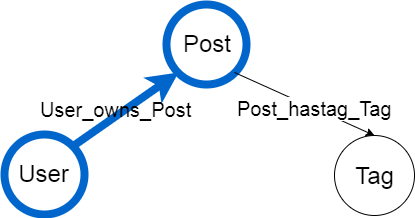
\includegraphics[scale=0.5]{pic/meta1.png}
\caption{\textit{Structure} of Query \#1}
\end{figure}



We say that (User)-[User\_owns\_post]-$>$(Post) is the structure of Query \#1.
The query is aggregated by (grouped by) user’s upvotes. We say that {User.Upvotes} is the dimension of Query \#1.
The query is aggregated on avarage of post’s score.  We say that {AVG(Post.Score)} is the meansure of Query \#1. 
 
Similarly, for Query \#2:

\textbf{Query \#2: 		Get average post score grouped by user’s upvotes and post’s post types. }

Structure:	(User)-[User\_ownspost]-(Post)

\begin {figure}[H]
\centering
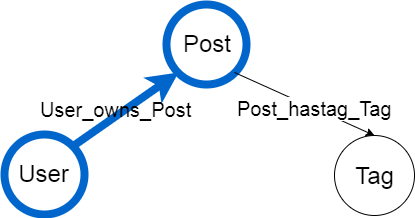
\includegraphics[scale=0.5]{pic/meta1.png}
\caption{\textit{Structure} of Query \#2}
\end{figure}

Dimensions:	{User.Upvotes, Post.PostTypeId}

Measures:	{AVG(Post.Score)}
 
Notice that Query \#2 adds Post.PostTypeId to Query \#1’s dimensions. That is to say, Query \#2 asks for a more detailed partitions over dimentions. We call Query \#2 a drill-down from Query \#1, and  Query \#1 a roll-up from Query \#2. Note that possible property combinations can be modeled as a lattice-structured cube. Figure 2.2 shows what a cube is like for properties \{A,B,C\}. We can see that roll-up and drill-down operations allow us to navigate up and down on a cube.


\begin {figure}[H]
\centering
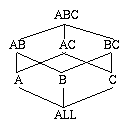
\includegraphics[scale=1]{pic/22.png}
\caption{Cube of properties \{A,B,C\}.}
\end{figure}

\textbf{Query \#3: 		Get average user age grouped by users’ 2017 posts’ tags.} 

Structure:	(User)-[User\_owns\_post]-(Post)-[Post\_hastag\_Tag]-(Tag)
\begin {figure}[H]
\centering
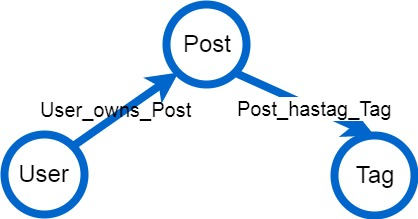
\includegraphics[scale=0.5]{pic/meta2.jpg}
\caption{\textit{Structure} of Query \#3}
\end{figure}


Dimensions:	{Tag.Tagname}

Measures:	{AVG(User.Age)}
 
Note that Query \#3 has different \textit{strucutre} than Query \#1 and Query \#2. In Query \#3, a requirement that post must be created in year 2017 picks out a particular subset of  all. In OLAP this is called ``slicing'' operation. Slicing operation allows users to view the data with filtering requirements on selected properties. 
 
In this thesis we call {Post.Year=2017} a \textit{``slicing condition''} of Query \#3.
 
To summarize, graph OLAP allows clients to aggregate different \textit{structures}, over different \textit{dimensions}, on different \textit{measures}, and optionally slice aggregation result by different \textit{slicing conditions}. Clients can change their views by performing roll-up, drill-down, and slicing freely and interactively.


%----------------------------------------------------------------------
\section{Graph Databases and Neo4j}
%----------------------------------------------------------------------


There are two major types of databases that store and process graph data: traditional relational databases and graph databases. 
 
Relational databases adopt traditional ways of modeling data in form of entity and relationship tables. For instance, for the following property graph, which consists 1 user and his or her 3 posts. A relational database stores the property graph as 3 tables:

\begin {figure}[H]
\centering
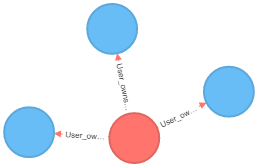
\includegraphics[scale=0.9]{pic/4.png}
\caption{A simple property graph.}
\end{figure}

Table-User
\begin{center}
\begin{tabular}{ l | l }  
	Uid	&{All user properties}	\\ \hline 
	1	&{Property values} \\
\end{tabular}
\end {center}

Table-Post
\begin{center}
	\begin{tabular}{ l | l }  
		Pid	& {All post properties}	\\ \hline 
		1	&{Property values} \\
		2	&{Property values} \\
		3	&{Property values} \\
	\end{tabular}
	\end {center}	
 
Table-Owns
\begin{center}
	\begin{tabular}{ l | l }  
		Uid	& Pid	\\ \hline 
		1	&1 \\
		1	&2 \\
		1	&3 \\
	\end{tabular}
	\end {center}

 
There are two drawbacks of storing property graphs in relational databases. First, each node or edge of in property graph could have arbitrary types of properties. However, schemas of relational tables restrict nodes or edges of a same type to have a uniform set of properties (attributes). Second and more importantly, edges are not stored as a separate table. For instance, we cannot directly query all the posts of a given user without joining User and Own tables in the above example.
 
Graph databases solve the above two issues by directly adopting property graph structures to store data. In graph databases, edges are stored not as independant tables but directly attached to related nodes using data structures such as adjacency lists. Many graph database applications have been implemented and commercialized. One of the popular ones is Neo4j.
 
Relational databases and graph databases both have their own strengths in term of query processing. However it is generally accepted that graph databases perform better at property graph data processing as it conforms more with the actual graph structure. 

Many graph database applications have been implemented and commercialized. One of the popular ones is Neo4j, which holds atomicity, consistency, isolation, durability (ACID). 
 
Instances are modeled and stored as  property graphs in Neo4j. Like other graph databases, edges are not stored as physically separate tables, but directly attached to their nodes. One special thing about Noe4j’s property graph is that its nodes and edges can be labeled with any number of labels (similar to entity and relationship types). For instance a node referring to a student could have various labels such as “student”, “people” etc. 

Cypher is Neo4j’s query language, which is expressive and simple. Here are some examples of Cypher queries:

Aggregation query: For answers(Post.PostTypeId=2), what is the average score group by different user upvotes?
 
match (u:User)-[r:User\_owns\_Post]-$>$(p:Post) where p.PostTypeId=`2' return u.Upvotes, AVG(p.Score)
 
Here “User” and “Post” are labels, PostTypeId and Score are properties of “Post” node, “Upvotes” is property of “User” node.
 
Neo4j is written in Java. While applications in various languages could interact the server by issuing queries and transport using BOLT protocol. BOLT protocol is a binary protocol implemented by Neo4j team. It is more efficient than HTTP protocol. 

%Figure 2.4 shows how applications interact with Neo4j server.
%
%\begin {figure}[H]
%\centering
%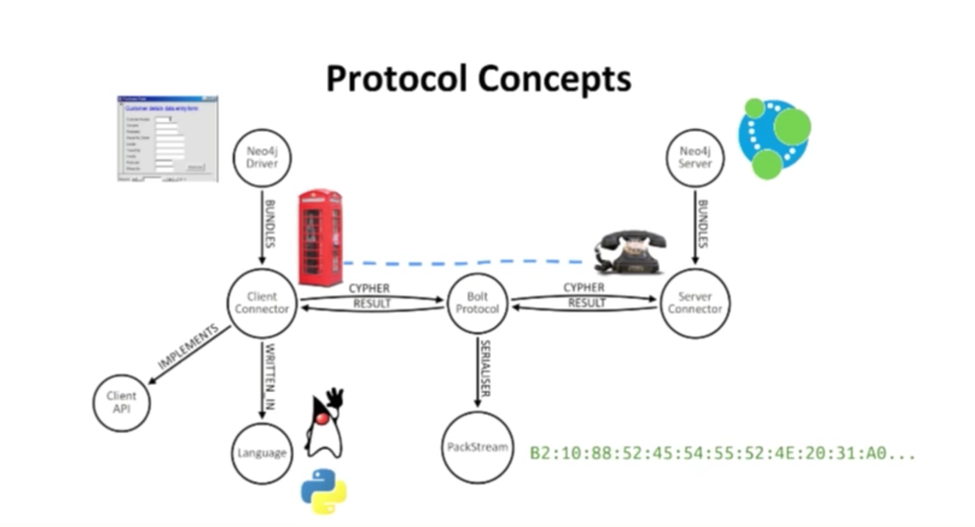
\includegraphics[scale=0.4]{pic/23.png}
%\caption{How applications interact with Neo4j server.}
%\end{figure}


%----------------------------------------------------------------------
\section{Related Work}
%----------------------------------------------------------------------

Numerous papers have been published on graph aggregation. 

Cube-based \cite{DBLP:conf/sofsem/JakawatFL16} proposes the concept of  graphs enriched by cubes. Each node and edge of the considered network are described by a cube. It allows the user to quickly analyze the information summa-
rized into cubes. It works well in slowly changing dimension problem in OLAP analysis.

Gagg \cite{DBLP:conf/esws/MaaliCD15} introduces an RDF graph aggregation operator that is both expressive and flexible. It provides a formal definition of Gagg on top of SPARQL Algebra and defines its operational semantics and describe an algorithm to answer graph aggregation queries. Gagg achieves significant improvements in performance compared to plain-SPARQL graph aggregation.

Pagrol \cite{DBLP:conf/icde/WangFWTAA14} provides an efficient MapReduce-based parallel graph
cubing algorithm, MRGraph-Cubing, to compute the graph cube
for an attributed graph. 

Graph Cube \cite{DBLP:conf/sigmod/ZhaoLXH11} introduces Graph Cube, a new data warehousing model that supports OLAP queries effectively on large multidimensional networks. It takes account of both attribute aggregation and structure summarization of the networks. In order to deal with “curse of dimensions”, a greedy algorithm framework is introduced for partial materialization of cuboids.

Graph OLAP \cite{DBLP:conf/icdm/ChenYZHY08} studies dimensions and measures in the graph OLAP scenario and furthermore develops a conceptual framework for data cubes on graphs. It differentiates different types of measures(distributive and holistic etc) by their properties during aggregation. It looks into different semantics of OLAP operations, and classifies the framework into two major subcases: informational OLAP and topological OLAP. It points out a graph cube can be fully or partially materialized by calculating a special kind of measure called aggregated graph. 


We summarize some of the most related ones as follows:
 \begin{table}
 	\small
 \begin{center}
 	\begin{tabular}{ | c | c | c | c | c |  } 
 		\hline 
 		 & Input graph & Query pattern & Layer structure & Highlight\\ \hline 
 		 Cube-based \cite{DBLP:conf/sofsem/JakawatFL16} & property graph & simple relation & yes & cubes on edges and nodes\\ \hline 
 		 Gagg \cite{DBLP:conf/esws/MaaliCD15} & property graph & all exact-match patterns & no & structural patterns\\ \hline 
 		 Pagrol \cite{DBLP:conf/icde/WangFWTAA14} & property graph & edge and node attributes & yes & Map-Reduce distributed computing\\ \hline 
 		 Graph Cube \cite{DBLP:conf/sigmod/ZhaoLXH11} & homogenous  & node attributes & yes & partial materialization algorithm\\ \hline 
 		 Graph OLAP \cite{DBLP:conf/icdm/ChenYZHY08} & property graph & edge and node attributes & yes & distributive and holistic measures\\ \hline 
 		 
 	\end{tabular}
 	\end {center}
 	\caption{Comparison }
\end{table}
 
 
From the summary we can categorize the papers into two kinds: 
 
First, like Graph Cube \cite{DBLP:conf/sigmod/ZhaoLXH11}, focuses on a simple subset of property graphs(e.g. graphs with only homogenous nodes and edges) and proposes optimizations in order to accelerate OLAP query processing. The optimizations are attribute-aware, and since the nodes and edges are of only one kind queries over different structures and structure-aware optimizations are out of the scope. 
 
Second, like Gagg \cite{DBLP:conf/esws/MaaliCD15}, focus on an abstract high-level framework that process generic queries over generic property graphs. However, query processing efficency is not studied.  
 
To conclude, we can see a lack of study on structure-aware optimizations for efficent graph OLAP. As mentioned in Section 1.3, efficency issue is one of the most challenging issues on graph OLAP. Therefore, it is very meaningful to explore faster structure-aware OLAP processing over general property graphs.



%----------------------------------------------------------------------
\section{Graph Cube}
%----------------------------------------------------------------------

In Graph Cube \cite{DBLP:conf/sigmod/ZhaoLXH11}, concepts of graph cube is introduced. Given a particular structure S, a property set P, and measure set M. We can aggregate over S on $2^{|P|}$ different combinations of dimensions. These $2^{|P|}$ queries can be mapped as a lattice structure, where each combination of dimensions corresponds to a cuboid in the lattice. We call the lattice structure of these $2^{|P|}$ queries a graph cube.


It has been pointed out in  Graph OLAP \cite{DBLP:conf/icdm/ChenYZHY08} that as long as if domain of measure is within \{count, sum, average\} and M contains count(*), the following feature holds:
 
Given any two cuboids C1 and C2 from the same graph cube, as long as dimension(C2) is a subset of dimension(C1), result of C1 can be used to generate result of C2. This is to say once a cuboid is materialized, all roll-up operations from this cuboid could be processed simply by scanning the materialized cuboid result. This will dramatically decrease roll-up operation time compared to aggregation from data graph(often of larger size, disk I/O), scanning materialized cuboid result(often of smaller size) is often much faster.


 
Ideally we can materialize all cuboids. But when number of dimension is large, number of cuboids grows exponentially, making total materialization impossible due to overwhelming space cost. To solve this Graph Cube \cite{DBLP:conf/sigmod/ZhaoLXH11} proposed a partial materialization algorithm on graph cube. It is a greedy algorithm and the score function is based on benefits of deduction of total computation cost.
